%%%%%%%%%%%%%%%%%%%% CHAPTER 3 %%%%%%%%%%%%%%%%%%%%%%%%%%
%%%%% Variables and Operators %%%%%%%%%%%%%%%%%%%%%%%%%%%%%%%%%%% 
\section{Interpolate Tabular Data}
Material properties in physical systems are usually tabulated values.
A frequent task is to interpolate in a set of tabular values to approximate the value between rows (or columns) in the table.  
Linear interpolation is the common technique used; and the tables can are stores as either separate files, or, if the tables are small enough, they can be directly imbedded into the code.

\subsection{Linear Interpolation}
Figure \ref{fig:XYPair} is a sketch of a set of ordered pairs $(x,y)$. 

\begin{figure}[h!] %  figure placement: here, top, bottom, or page
   \centering
   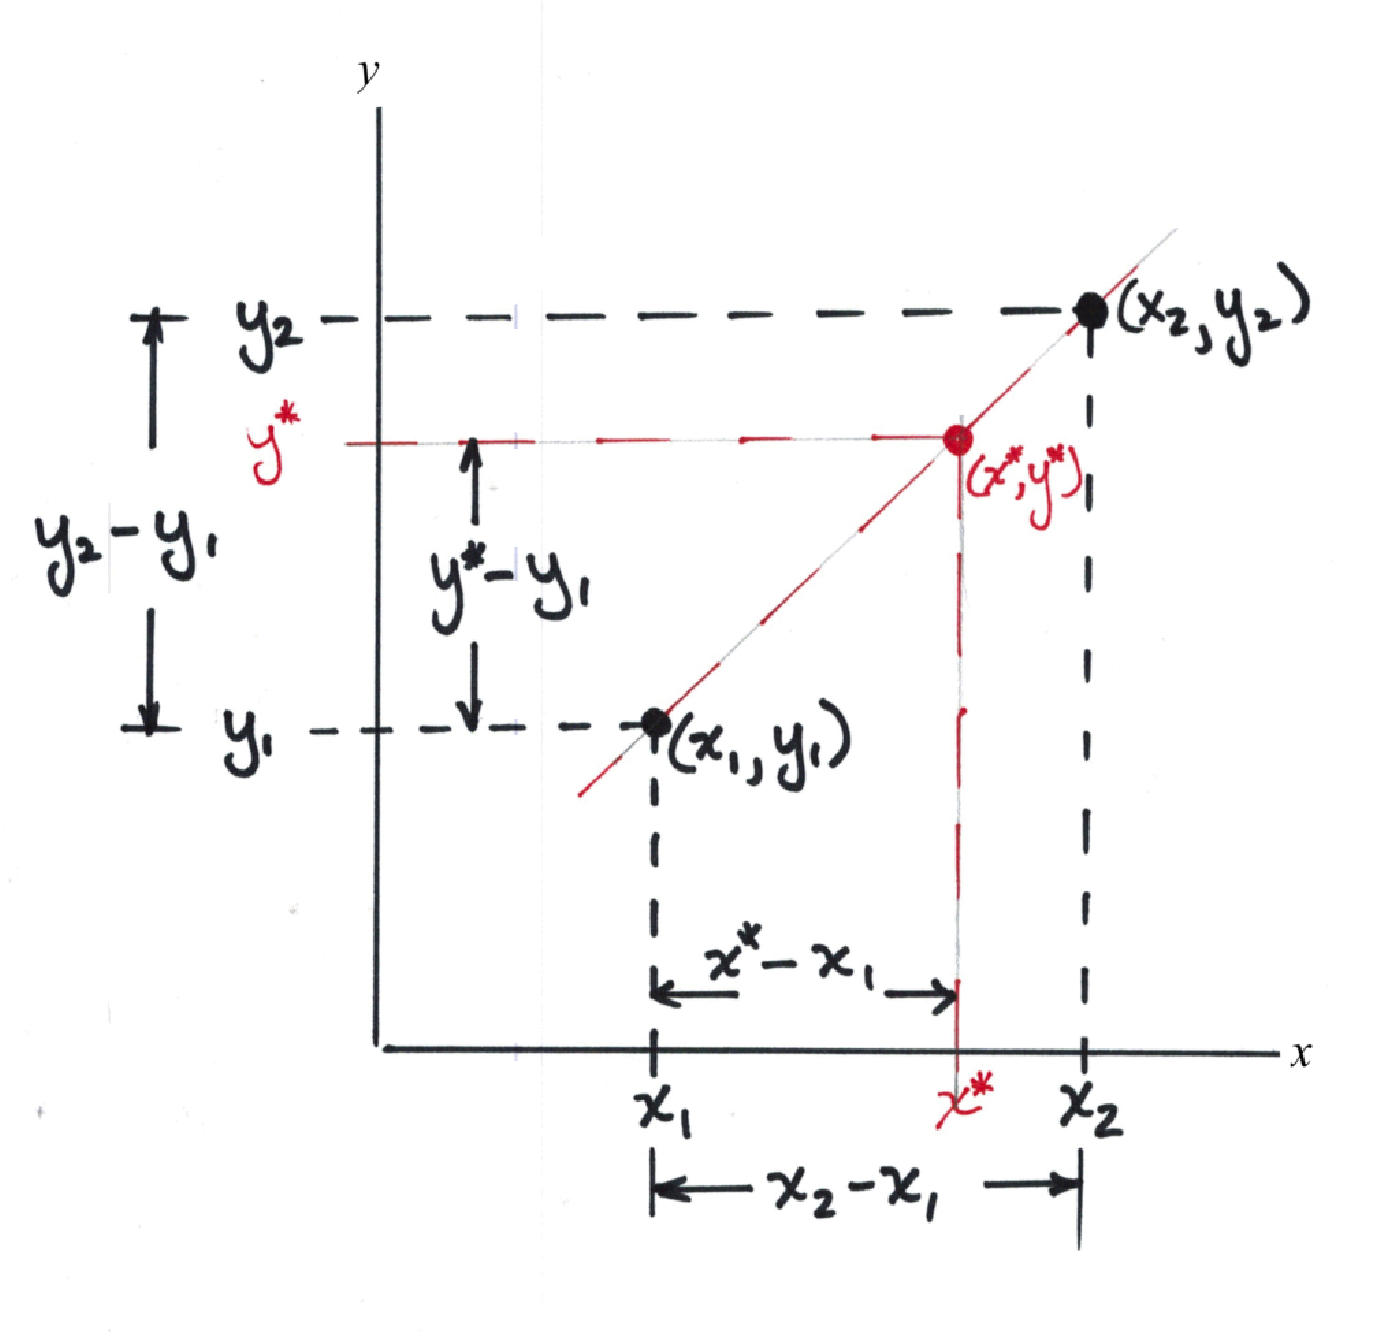
\includegraphics[width=6in]{./3-InterpolateTabular/XYPair.jpg} 
   \caption{Sketch of two adjacent values from a table, plotted in Cartesian coordinate system.}
   \label{fig:XYPair}
\end{figure}

These pairs (there are two in the sketch) represent values in a table, for instance $x$ may represent water temperature, and $y$ may represent vapor pressure at that particular temperature.
Two adjacent values (in the table) are depicted in the sketch, and the pairs are ordered bases on the $x$-value.  

Now suppose we want to estimate the value of $y^*$ at some intermediate value $x^*$ that lies between $x_1$ and $x_2$.
As a computational task, the problem statement is to\\~\\
``Estimate the value of $y^*$ associated with the value $x^*$ given the ordered pairs $(x_1,y_1)$ and $(x_2,y_2)$.'' \\~\\
Linear interpolation simply uses the concept of similar triangles to scale the $x$ and $y$ distances between the ordered pairs to the intermediate location.   Equation \ref{eqn:InterpolationEquation} is the result of application of similar triangles to the situation described by Figure \ref{fig:LinearInterpolation} and the problem statement.

\begin{equation}
\frac{x^*-x_1}{x_2-x_1}=\frac{y^*-y_1}{y_2-y_1}
\label{eqn:InterpolationEquation}
\end{equation}

Next, apply algebra to solve Equation \ref{eqn:InterpolationEquation} for $y^*$, to obtain Equation \ref{eqn:InterpolationEquation2}

\begin{equation}
y^*=y_1+\frac{(y_2-y_1)(x^*-x_1)}{(x_2-x_1)}
\label{eqn:InterpolationEquation2}
\end{equation}

Now we can use \ref{eqn:InterpolationEquation2} to estimate values between any two data pairs.\\

\subsubsection{Interpolation of Values in Two Pairs}

Figure \ref{fig:FluidData} is a table of water properties from (CITE), that represents typically how tabular data are presented.  The temperature column is arranged in increasing order and the other properties associate with temperature across a row.

\begin{figure}[htbp] %  figure placement: here, top, bottom, or page
   \centering
   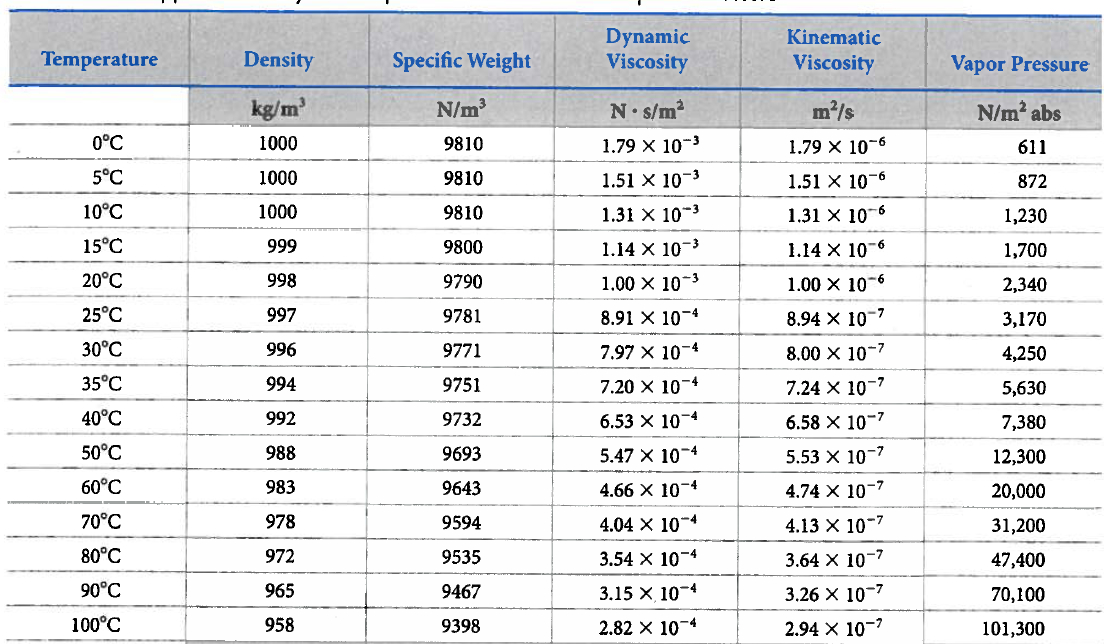
\includegraphics[width=6in]{./3-InterpolateTabular/FluidData.jpg} 
   \caption{Table of water properties in SI units (from CITE)}
   \label{fig:FluidData}
\end{figure}

Now suppose we wished to estimate the density of water at $44^o$ C.  
The two ordered pairs of temperature and density that surround $44^o$ C are $(40^o~C,992~kg/m^3)$ and $(50^o~C,988~kg/m^3)$.
So, to estimate the unknown density we can apply Equation \ref{eqn:InterpolationEquation2} and obtain the following result
\begin{equation}
y^*=992+\frac{(988-992)(44-40)}{(50-40)}=990.4
\label{eqn:DensityInterpolation}
\end{equation}

We might want to do this a lot, so we could write a simplistic script in R and remember to load it into our environment when we need it

\begin{lstlisting}[caption=R code demonstrating the interpolation equation, label=lst:InterpolatePairs]
# EXAMPLE # ** Interpolating Between Tabulated Pairs
interpolate2pairs<-function(xstar,x1,y1,x2,y2){
# apply interpolation equation
#   does not trap errors (divide by zero, etc)
  ystar <- y1 + (y2-y1)*(xstar-x1)/(x2-x1)
  return(ystar)
}
# In R Console
> interpolate2pairs(44,40,992,50,988)
[1] 990.4
> 
\end{lstlisting}   

For a single interrogation of a table we can stop here, but in many instances we have to interrogate a table a lot -- we want some kind of program structure to handle the work so all we have to do is pass the temperature value and have the program return the density.

\subsubsection{Interpolation of Values in Two Arrays}
To accomplish repeated interpolation we will need to have: (1) an interpolating method (we have the beginning of one above in Listing \ref{lst:InterpolatePairs}), (2) the entire table so we don't have to enter the pairs, and (3) a way to  automatically search the table so we don't have to look up values and supply them to the interpolator.

The table itself in this instance is relatively small, so we can simply assign values to some constant arrays in below in Listing \ref{lst:AssignFluidConstants}.

\begin{lstlisting}[caption=R code assigning Liquid Properties, label=lst:AssignFluidConstants]
# EXAMPLE # ** Assigning Constants
tempSI<-c(0.00,5.00,10.00,15.00,20.00,25.00,30.00,35.00,
   40.00,50.00,60.00,70.00,80.00,90.00,100.00)
densitySI<-c(1000.00,1000.00,1000.00,999.00,998.00,997.00,996.00,
   994.00,992.00,988.00,983.00,978.00,972.00,965.00,958.00)

# In R Console
> cbind(tempSI,densitySI)
      tempSI densitySI
 [1,]      0      1000
 [2,]      5      1000
 [3,]     10      1000
 [4,]     15       999
 [5,]     20       998
 [6,]     25       997
 [7,]     30       996
 [8,]     35       994
 [9,]     40       992
[10,]     50       988
[11,]     60       983
[12,]     70       978
[13,]     80       972
[14,]     90       965
[15,]    100       958
> 
\end{lstlisting}  

Returning to our example, the value $44$ lies between \texttt{tempSI[9]} and \texttt{tempSI[10]}, so we desire an algorithm that starts at \texttt{tempSI[1]} and determines if the search value is between \texttt{tempSI[1]} and \texttt{tempSI[2]}, if not, then increment the row counter and determine if the search value is between \texttt{tempSI[2]} and \texttt{tempSI[3]}, and so on.

Once we locate in the searched array where the value lies then the interpolation uses the lower and upper elements of the range to interpolate.  In the case of our example, once we determine the $44$ lies between  \texttt{tempSI[9]} and \texttt{tempSI[10]}, then the interpolation equation is

\begin{equation}
y^*=\texttt{densitySI[9]}+\frac{(\texttt{densitySI[10]}-\texttt{densitySI[9]})(44-\texttt{tempSI[9]})}{(\texttt{tempSI[10]}-\texttt{tempSI[9]})}
\label{eqn:InterpolationArrayEquation}
\end{equation}

Listing \ref{lst:GetAValue} is an \textbf{R} script that implements the search and interpolation just described.  The script assumes that the searched array ($x$) is ordered and increasing -- not a trivial assumption!  The script has some limited error handling to test if the search value actually lies in the total range of the array before beginning the search.  Once these tests are passed, then the code searches in the $x$ array for the search value $x^*$ and finds the two rows that contain the value.  Once the rows are located, the interpolation equation is used.

\begin{lstlisting}[caption=R code to Search and Interpolate, label=lst:GetAValue]
# EXAMPLE # ** Search and Interpolate
  getAvalue <- function(x,xvector,yvector){
    # returns a y value for x interpolated from (xvector,yvector)
    # xvector is assumed to be in a monotonic sequence
    # function performs limited error checks
    # NULL return is error indicator
    # T.G. Cleveland July 2007 
    #
    xvlength <- length(xvector)
    yvlength <- length(yvector)
    # check that vector lengths same
    if(xvlength != yvlength){
      message("vectors xvector and yvector different lengths -- exiting function")
      return()
    }
    # check that x in range xvector
    if(x < min(xvector)){
      message(" x too small -- exiting function")
      return()
    }
    if(x > max(xvector)){
      message(" x too big -- exiting function")
      return()
    }
    #
    for (i in 1:(xvlength-1)){
      if( (x >= xvector[i]) & (x < xvector[i+1]) ){
        result = yvector[i]+(yvector[i+1]-yvector[i])*(x - xvector[i])/
        (xvector[i+1]-xvector[i])
        return(result)
      }
      # next row  
    }
    # check if at endpoint
    if( (x >= xvector[xvlength-1]) & (x <= xvector[xvlength]) ){
      result = yvector[i]+(yvector[i+1]-yvector[i])*(x - xvector[i])/
      (xvector[i+1]-xvector[i])
      return(result)
    }
    # should never get to next line
    message("something is really wrong -- check the vectors!")
    return()
  }
 # In R Console:  
> getAvalue(44,tempSI,densitySI)
[1] 990.4
> 
  \end{lstlisting}  

Now we can load and run the \texttt{getAvalue} script and supply the two vectors plus the search value as shown in Listing \ref{lst:GetAValue}

This look-up process is readily transferred to other cases, we do have to decide if the data will be coded as constants (as was done here) or read from a file -- if the database is large the file read option is best.  In terms of building a generic look-up tool several things actually happen in a particular order.

\begin{enumerate}
\item The function call loads in the table (of reading from a file, we would have to forward declare the vectors).
\item The function searches the first vector for the bounding location of the search variable.
\item Once the boundaries are located, the interpolation is performed -- notice how the last boundary pair is handled.
\end{enumerate}

Now we can combine the data assignment, the search and interpolate into a single function so when we want to evaluate in the future we only need the single function.

Listing \ref{lst:getDensitySI} is an example of everything combined.   Here I have embedded the \texttt{getAvalue} script into the function so the whole function itself is portbable (we don't have keep track of \texttt{getAvalue}).  This embedding can be replaced with a load from a library (but then we must keep track of the path).  

The library way is preferable; if \texttt{getAvalue} needs changing, we will have to change every instance of it in the code, if we miss one the code may still run and it could be years before we discover the error because a single instance of code fragment within a larger code was missed -- its far better to only change a single instance of the function when maintenance is necessary.

\begin{lstlisting}[caption=R code to Return Water Density for Given Temperature, label=lst:getDensitySI]
# Script to return water density in SI units as a function of temperature
getDensitySI<-function(t){
# load the getAvalue() function ###################################################
  getAvalue <- function(x,xvector,yvector){
    # returns a y value for x interpolated from (xvector,yvector)
    # NULL return is error indicator
    #
    xvlength <- length(xvector)
    yvlength <- length(yvector)
    # check that vector lengths same
    if(xvlength != yvlength){
      message("vectors xvector and yvector different lengths -- exiting function")
      return()
    }
    # check that x in range xvector
    if(x < min(xvector)){
      message(" x too small -- exiting function")
      return()
    }
    if(x > max(xvector)){
      message(" x too big -- exiting function")
      return()
    }
    #
    for (i in 1:(xvlength-1)){
      if( (x >= xvector[i]) & (x < xvector[i+1]) ){
        result = yvector[i]+(yvector[i+1]-yvector[i])*(x - xvector[i])/
          (xvector[i+1]-xvector[i])
        return(result)
      }
      # next row  
    }
    # check if at endpoint
    if( (x >= xvector[xvlength-1]) & (x <= xvector[xvlength]) ){
      result = yvector[i]+(yvector[i+1]-yvector[i])*(x - xvector[i])/
        (xvector[i+1]-xvector[i])
      return(result)
    }
    # should never get to next line
    message("something is really wrong -- check the vectors!")
    return()
  }
#########################################################################################
# load the data vectors, tempSI and densitySI
tempSI<-c(0.00,5.00,10.00,15.00,20.00,25.00,30.00,35.00,
  40.00,50.00,60.00,70.00,80.00,90.00,100.00)
densitySI<-c(1000.00,1000.00,1000.00,999.00,998.00,997.00,996.00,
  994.00,992.00,988.00,983.00,978.00,972.00,965.00,958.00)
# now call getAValue
result<-getAvalue(t,tempSI,densitySI)
return(result)
}
  \end{lstlisting}  

The ``library'' approach is demonstrated in Listing \ref{lst:PlotDensity}; in this listing the path in the \texttt{source()} command is unique to my machine -- your path is likely to be different.  I find it is useful to contain all the various codes into a single directory and source that directory once to find the path, then change all the source calls to that path.  In fact that path can be a string variable and the referencing can be automatic (as long as the files exist!).

Once the look-up function is built then we can  interrogate the table many times; and even build a plot of the table -- these features are demonstrated in Listing \ref{lst:PlotDensity}.

\begin{lstlisting}[caption=R code demonstrating use of getDensitySI(), label=lst:PlotDensity]
## In R Console  
> # Example demonstrating use of functions
> # load in the functions (must exist -- use path on your machine)
> source('~/Dropbox/1-CE-TTU-Classes/UnderDevelopment/
   CE4333-PCH-R/6-RScripts/getAvalue.R')
> source('~/Dropbox/1-CE-TTU-Classes/UnderDevelopment/
   CE4333-PCH-R/6-RScripts/getDensitySI.R')
> # Now use them
> getDensitySI(44)
[1] 990.4
> getDensitySI(54)
[1] 986
> getDensitySI(88)
[1] 966.4
> t<-seq(0,100,2) # make a temperature vector 0 to 100 in 2 degree increments
> d<-numeric(0) # forward declare d to store results
> howMany<-length(t)
> for(i in 1:howMany){
+     d[i]<-getDensitySI(t[i])
+ }
> plot(t,d,type="l",xlab="Degrees Celsius",ylab="Density (kg/m^3)")
> 
\end{lstlisting}  

The resulting plot is shown on Figure \ref{fig:PlotDensity} below.
\begin{figure}[htbp] %  figure placement: here, top, bottom, or page
   \centering
   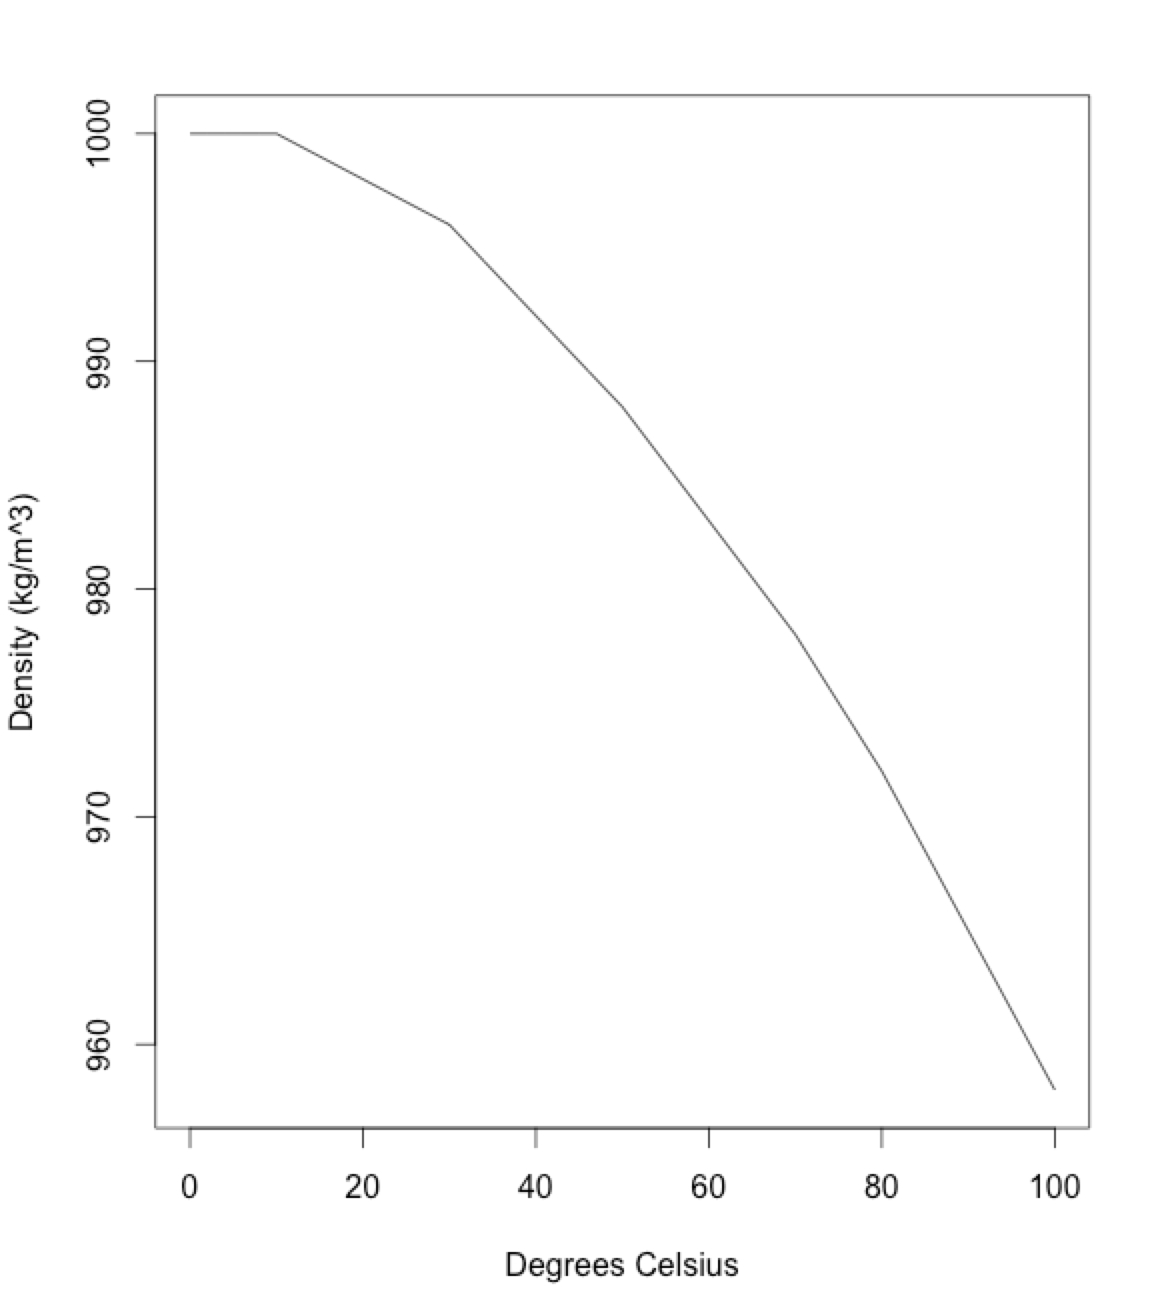
\includegraphics[width=5in]{./3-InterpolateTabular/PlotDensity.jpg} 
   \caption{Plot of density versus temperature generated using the \texttt{getDensity()} function.}
   \label{fig:PlotDensity}
\end{figure}



\subsection{Exercises}
\begin{enumerate}
\item Build a function \texttt{getDensityUS()} that searches the table in Figure \ref{fig:FluidData} and returns the density of water in US customary units for a value of temperature supplied in degrees Farenheight. \\~\\
Submit your code and screen captures of the density for temperatures of $43^o~F$, $146^o~F$, and $210^o~F$.

\item Later in the class we will need functions to return viscosity to compute head losses in pipe networks.  \\

 Build and test a function \texttt{getKinViscosityUS()} that searches the table in Figure \ref{fig:FluidData} and returns the kinematic viscosity of water in US customary units for a value of temperature supplied in degrees Farenheight\\~\\
Submit the code and screen captures of the kinematic viscosity for temperatures of $43^o~F$, $146^o~F$, and $210^o~F$. 

\item Build and test a function \texttt{getKinViscositySI()} that searches the table in Figure \ref{fig:FluidData} and returns the kinematic viscosity of water in SI units for a value of temperature supplied in degrees Celsius \\~\\
Submit the code and screen captures of the kinematic viscosity for temperatures of $13^o~C$, $66^o~C$, and $97^o~C$.
\end{enumerate}
%%%%%%%%%%%%%%%%%%%%%%%%%%%%%%%%%%%%%%%%%%%%%%%%%%%%%%%%%%%%%%%